\documentclass[conference]{IEEEtran}
% \IEEEoverridecommandlockouts
% The preceding line is only needed to identify funding in the first footnote. If that is unneeded, please comment it out.
\usepackage{cite}
\usepackage{amsmath,amssymb,amsfonts}
\usepackage{algorithmic}
\usepackage{graphicx}
\usepackage{textcomp}
\usepackage{xcolor}
\def\BibTeX{{\rm B\kern-.05em{\sc i\kern-.025em b}\kern-.08em
    T\kern-.1667em\lower.7ex\hbox{E}\kern-.125emX}}
% Definiciones propias
\usepackage{comandos}

\begin{document}

\title{
Authentication codes  \\
{\footnotesize Information security proposal for 2022 Wolfram summer school}
}

\author{
    \IEEEauthorblockN{Armando Benjamín Cruz Hinojosa}
    \IEEEauthorblockA{
        \textit{Universidad Nacional Autónoma de México}\\
        Mexico City, Mexico \\
        aleph\_g@ciencias.unam.mx
    }
}

\maketitle

\begin{abstract}
    Current authentication schemes are based on asymmetric cryptography protocols like RSA, with the arrival of quantum computing and fast factorization algorithms, security is endangered. A-schemes presents an alternative that remains secure regardless of computational power, but there are no tools to measure how secure they are. This proposal intends to create such tool.
\end{abstract}

% \begin{IEEEkeywords}
%     component, formatting, style, styling, insert
% \end{IEEEkeywords}

%
% Introduction
%
\section{Introduction}
Authentication is a fundamental aspect of information security, it provides protection against impersonations and false messages. A strategy implemented in a communication system to achieve such protection is called an \textit{authentication scheme}.

An authentication scheme is said to be secure if the if the chance that an impostor fools the system is so small that it doesn't represent a risk in the communication (comparable to channel noise).

A common scheme is to add a \textit{digital signature} at the end of each message. This signature is generated with asymmetric cryptography: The message is compressed to a fixed size with a cryptographic hash function (like SHA-256), this hash is then encrypted with the transmitter's private key. In order to verify the message, the receiver compares the message's hash with the decrypted signature if they differ the message is forged.

Without the private key the best the enemy can do is try different keys until the message is accepted. This takes $2^{n-1}$ tries on average ($n$ is the size of the key). HTTPS specifies a maximum key size of 2048 bits and RSA encryption. A brute force attack would take $2^{2047} \approx 10^{616}$ tries, impossible task for current computers.

But if an efficient solution to the factorization into prime factors is used to break the key (Shor's algorithm \cite{b1}) or if the impostor's computational power drastically increases, the digital signature is useless for authentication protection.

With this in mind \cite{b2} proposes a different kind of authentication schemes, called \textit{A-schemes}, that remains secure regardless of the impostor's computational power. Three parts interact in the communication system: \A\ an information source that wishes to communicate an element of the set of all possible source states $\s$, \B\ a receiver and \E\ the impostor.

\A\ will transform the source states into \textit{ciphered messages} (sequences compatible with the communication channel) by means of an \textit{encoding rule}. An encoding rule $r\in\r$ is a one-to-one mapping from $\s$ to $\m$. \B\ accepts a message $m$ as authentic if $m\in r[\s]$ and retrieves the original state with the pre-image $r^{-1}(m)$. This schema is represented in Figure~\ref{figModelo3Participantes}.

\begin{figure}
    \centering
    \resizebox{4.5px}{!}{
        \begin{tikzpicture}[trim left=(channel), trim right=(channel), auto, node distance=2cm,>=latex, scale=0.50]
            \node [smallblock](channel){};
            \node [block, left of=channel, node distance=3cm, label=below:Encoder](encoder){$ \r $};
            \node [block, left of=encoder, node distance=3cm, label=below:{\parbox{6em}{\centering Information\\source}}](infosource){\A};
            \node (decoder)[block, right of=channel, node distance=3cm, label=below:Decoder]{};
            \node (destination)[block, right of=decoder, node distance=3cm, label=below:Receiver]{\B};
            \node (enemy)[block, below of=channel, label=below:Impostor]{\E};

            \draw [->] (infosource) -- node[name=u]{\parbox{1.5cm}{\centering \textit{source state}}} (encoder);
            \draw [->] (encoder) -- node {\parbox{2cm}{\centering \textit{cyphered message}}} (channel);
            \draw [->] (channel) -- node {\parbox{2cm}{\centering \textit{received message}}} (decoder);
            \draw [->] (decoder) -- node [name=y]{\parbox{1.5cm}{\centering \textit{source state}}}(destination);
            \draw [->] (enemy) -- node[name=enemychannel]{} (channel);
            \node [left of=enemychannel, node distance=7mm]{\parbox{2cm}{\centering \textit{forged message}}};
        \end{tikzpicture}
    }
    \caption{A-scheme communication system.}
    \label{figModelo3Participantes}
\end{figure}

An A-schema is a 5-tuple $\aprottuple$, where $\ped{S}$ denotes a stochastic process over the set of all source states ie. the \textit{information source}, and $\pr$ is the probability distribution over the set of encoding rules. An \textit{A-code} is the 3-tuple $\acodetuple$ also referred as the A-scheme's combinatorial structure.

The impostor's best strategy is to listen to the first $t$ ciphered messages and with a cryptanalytical analysis, forge a message with the highest probability of success. The \textit{unconditional probability of success of order $t$} ($P_t$) is the expected percentage of successfully spoofed messages.

$P_t$ is the measurement of the security of an A-scheme, \cite{b3} demonstrates the theoretical lower bound for the unconditional probability of success, in terms of information entropy:
\[
    P_t \geq
    e^{
    \hc{R\;\;}{\;M^{t+1}}
    - \hc{R\;\;}{\;M^{t}}
    }
\]

Finally \cite{b4} characterizes the A-schemes that achieve the theoretical lower bound. Such schemes satisfy two conditions.
\begin{itemize}
    \item The information source $\ped{S}$ is message uniform.
    \item The underlying A-code structure is a strong partially balanced $t$-design (SPBD).
\end{itemize}

%
% Objective
%
\section{Objective}
The unconditional probability of success is the \textit{expected} percentage of successfully spoofed messages. However very little is known about the probability distribution and variance of this random process.

On the other hand, the caracterization of perfect A-schemes imposes a restriction over the information source ($\ped{S}$ must be message uniform), that most information sources don't meet. Several unknown questions rise:
\begin{itemize}
    \item How much $P_t$ differs from its theoretical lower bound, given an A-schemes with non message uniform source?
    \item Are SPBD the best A-code structure for such schemes?
\end{itemize}

Insight is needed to solve both problems. My proposal's objective is to implement in Wolfram language, a pseudo random simulation tool of the impostor's strategy, that will allow to generate data to statistically describe the spoof percentage, distribution and variance.

The simulations will be done over distinct information sources and distinct A-codes, focusing on the two questions related to non message uniform information sources.

%
% Implementation
%
\section{Implementation}
Once the data points are generated, using Wolfram's \textit{least square fitting} regression will describe the distribution and variance. Using Wolfram's descriptive statistics and plotting functionality, I hope to find a relation on the difference to the theoretical lower bound, in the non perfect A-schemes, this will lead to a mathematical hypothesis.

The problem lies in generating the data points ie. the simulation. This simulation must be as unbiased as possible, and optimal in order to generate a lot of data in short time. In order to achieve the simulation algorithm two things are needed.

\subsection{Information source simulation}
Shannon defines an information source as a family of random variables dispensing sequences words in time: a discrete stochastic process over the set of all source states.

Last year, Mythreyi Namuduri's Wolfram summer school project \cite{b6}, showed this statistical nature of language, by listing the most common words for less commonly spoken languages.

Wolfram's WordList function together with a Markov chain and a random number generator can be used to simulate an information source on a particular language.

\subsection{A-codes and SPBDs}
A block design (Fig~\ref{block_design}) is a specific type of hypergraph that can be defined in Wolfram language as a list of sets of vertices. On the other hand, an A-code is a list of two sets and a family of one-to-one mappings from the first set to the second one, something that can be defined in Wolfram's language as a relation.

\begin{figure}[htbp]
    \centerline{
        \scalebox{.48}{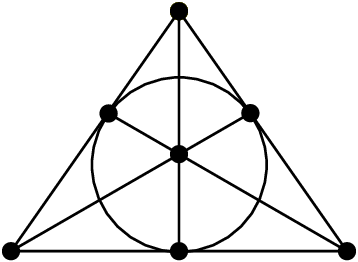
\includegraphics{block-design.png}}
    }
    \caption{Example of combinatorial block design.}
    \label{block_design}
\end{figure}

\cite{b4} characterization of perfect schemes gives an algorithm to transform a given SPBD into an A-code. This will be implemented as a function that takes an SPBD block design, the set of source states and the set of encoding messages and returns an A-code.

\newpage
%
% Familiarity with the problem
%
\section{Familiarity with the problem}
I have been working with A-schsemes and A-codes for over a year for my bachelor degree's thesis (all UNAM's Math bachelors must present a thesis).

The content of the thesis is a proof (and explanation) of the theoretical lower bound described above, and a poof (and explanation) of the characterization of perfect A-schemes in terms of SPBDs block designs.

%
% Bibliografía
%
\begin{thebibliography}{00}
    \bibitem{b1} G. Eason, B. Noble, and I. N. Sneddon, ``On certain integrals of Lipschitz-Hankel type involving products of Bessel functions,'' Phil. Trans. Roy. Soc. London, vol. A247, pp. 529--551, April 1955.
    \bibitem{b2} J. Clerk Maxwell, A Treatise on Electricity and Magnetism, 3rd ed., vol. 2. Oxford: Clarendon, 1892, pp.68--73.
    \bibitem{b3} I. S. Jacobs and C. P. Bean, ``Fine particles, thin films and exchange anisotropy,'' in Magnetism, vol. III, G. T. Rado and H. Suhl, Eds. New York: Academic, 1963, pp. 271--350.
    \bibitem{b4} K. Elissa, ``Title of paper if known,'' unpublished.
    \bibitem{b5} R. Nicole, ``Title of paper with only first word capitalized,'' J. Name Stand. Abbrev., in press.
    \bibitem{b6} Y. Yorozu, M. Hirano, K. Oka, and Y. Tagawa, ``Electron spectroscopy studies on magneto-optical media and plastic substrate interface,'' IEEE Transl. J. Magn. Japan, vol. 2, pp. 740--741, August 1987 [Digests 9th Annual Conf. Magnetics Japan, p. 301, 1982].
    \bibitem{b7} M. Young, The Technical Writer's Handbook. Mill Valley, CA: University Science, 1989.
\end{thebibliography}

\end{document}
